\section{実験結果}

\subsection{設計指標における成功率の算出結果}
設計指標の算出に必要なエンドエフェクタモデルのパラメータを\tabref{Tab:modelparam}に示す.

\begin{table}[H]
  \begin{center}
    \scalebox{0.8}{
    \begin{tabular}{l|cccccc}
      Model & $S_f$ [$mm^2$] & $d_fside$ [$mm$] & $d_fabove$ [$mm$] & $d_fbelow$ [$mm$] & $S_p$ [$mm^2$]& $d_p$ [$mm$]\\ \hline\hline
      Gripper type & 415.6 & 72.7 & - & - & 15.4 & 38.2\\
      Vibrating knife type & - & - & 75.1 & 67.9 & 11.6 & 20\\
      Peduncle approach type & - & - & - & - & 51.7 & 9\\
    \end{tabular}
    }
    \caption{Parameters of the end effector models}
    \label{Tab:modelparam}
  \end{center}
\end{table}

エンドエンドエフェクタモデルがアプローチに成功するかの推測結果を \tabref{Tab:resultindicators1} \verb|〜| \tabref{Tab:resultindicators3} に示す.
設計指標から成功率を求めた結果を\tabref{Tab:successrateindicators}に示す.

\begin{table}[H]
  \begin{center}
    \begin{tabular}{l|ccccc}
      ID & $d_p > l_p$ & $S_p > S_papproach$ & $d_fside > l_fside$ & $S_f > S_fapproach$ & success\\ \hline\hline
      2 & × & ○ & × & × & ×\\
      4 & × & ○ & × & ○ & ×\\
      5 & × & ○ & × & ○ & ×\\
      7 & ○ & ○ & ○ & ○ & ○\\
      9 & × & ○ & × & ○ & ×\\
      10 & × & ○ & × & ○ & ×\\
      11 & × & ○ & × & ○ & ×\\
      13 & × & ○ & × & ○ & ×\\
      14 & × & ○ & × & ○ & ×\\
      20 & × & × & × & × & ×\\
      22 & ○ & ○ & ○ & ○ & ○\\
      30 & × & ○ & × & ○ & ×\\
    \end{tabular}
    \caption{Results from design indicators ① gripper type}
    \label{Tab:resultindicators1}
  \end{center}
\end{table}

\begin{table}[H]
  \begin{center}
    \begin{tabular}{l|ccccc}
      ID & $d_p > l_p$ & $S_p > S_papproach$ & $d_fabove > l_fabove$ & $d_fbelow > d_fbelow$ & success\\ \hline\hline
      2 & ○ & ○ & ○ & ○ & ○\\
      4 & × & ○ & × & × & ×\\
      5 & × & ○ & × & × & ×\\
      7 & ○ & ○ & × & ○ & ×\\
      9 & × & ○ & × & ○ & ×\\
      10 & × & ○ & × & × & ×\\
      11 & × & ○ & × & × & ×\\
      13 & × & ○ & × & ○ & ×\\
      14 & × & ○ & × & ○ & ×\\
      20 & × & × & × & × & ×\\
      22 & ○ & ○ & × & ○ & ×\\
      30 & × & ○ & × & ○ & ×\\
    \end{tabular}
    \caption{Results from design indicators ② vibrating knife type}
    \label{Tab:resultindicators2}
  \end{center}
\end{table}

\begin{table}[H]
  \begin{center}
    \begin{tabular}{l|ccccc}
      ID & $d_p > l_p$ & $S_p > S_papproach$ & success\\ \hline\hline
      2 & ○ & ○ & ○\\
      4 & × & × & ×\\
      5 & × & × & ×\\
      7 & ○ & ○ & ○\\
      9 & × & ○ & ×\\
      10 & × & × & ×\\
      11 & × & × & ×\\
      13 & × & × & ×\\
      14 & × & × & ×\\
      20 & × & × & ×\\
      22 & ○ & ○ & ○\\
      30 & ○ & ○ & ○\\
    \end{tabular}
    \caption{Results from design indicators ③ peduncle approach type}
    \label{Tab:resultindicators3}
  \end{center}
\end{table}

\begin{table}[H]
  \begin{center}
    \begin{tabular}{l|ccc}
      Model & Gripper type & Vibrating knife type & Peduncle approach type\\ \hline\hline
      Number of success & 2/12 & 1/12 & 4/12\\
    \end{tabular}
    \caption{Success rate from design indicators}
    \label{Tab:successrateindicators}
  \end{center}
\end{table}

\subsection{実環境における成功率の結果}
実環境でのアプローチの実験結果を\tabref{Tab:successrateexperiment}に示す.
花柄アプローチ型, グリッパ型, 振動ナイフ型の順に成功率が高かった.
花柄アプローチ型に関して, 9回成功のうち3回は障害物に接触したが失敗条件を満たさなかったため成功とした.

\begin{table}[H]
  \begin{center}
    \begin{tabular}{l|ccc}
      Model & Gripper type & Vibrating knife type & Peduncle approach type\\ \hline\hline
      Number of success & 2/30 & 0/30 & 9/30\\
    \end{tabular}
    \caption{Success rate from experiment}
    \label{Tab:successrateexperiment}
  \end{center}
\end{table}

\subsection{成功率の比較}
\tabref{Tab:successrateindicators}と\tabref{Tab:successrateexperiment}から, アプローチの成功数は異なるものの, 各エンドエフェクタにおける成功率の傾向は似ていることがわかる.
\tabref{Tab:comparisonrate}は設計指標から推定したアプローチの可否と実環境でのアプローチの可否を比較している表である.
グリッパ型は推定結果と実際の結果が一致しているが, 振動ナイフ型と花柄アプローチ型は一致していない部分がある.
ID:2のピーマンに注目すると, \figref{Fig:id2}のように本来は花柄の前に茎が横切るような形で位置しているが, \figref{Fig:id2model}に示すID:2の3Dモデルをみると茎が欠損していることがわかる.
このことから果実がうまく3Dモデル化できていないため, 正しい障害物間距離を計測できずに間違った結果を推定してしまったのではないかと考える.
また, ID:11やID:14のときの花柄アプローチ型は, 実環境での実験では成功しているのに設計指標からの推定では失敗している.
設計指標からの推定結果である\tabref{Tab:resultindicators3}によると, 失敗の原因は, 花柄側面障害物間距離が許容範囲ではないことと, 花柄アプローチ面積よりも花柄が露出していないことである.
露出面積が少ないことは, 先ほど同様花柄が欠損している可能性がある.
障害物間距離に関して, この実験では花柄へアプローチする位置に関しては明確に設定できていないため, 花柄の一部が障害物に近いと, アプローチできる空間があっても失敗としてしまっていることが原因ではないかと考える.

\begin{table}[H]
  \begin{center}
    \scalebox{0.83}{
    \begin{tabular}{l|ccc|ccc|}
         & \multicolumn{3}{|c|}{Experiment} & \multicolumn{3}{|c|}{Design indicators}\\ \hline
      ID & Gripper & Vibrating knife & Peduncle approach & Gripper & Vibrating knife & Peduncle approach\\ \hline\hline
      2 & × & × & ○ & × & ○ & ○\\
      4 & × & × & × & × & × & ×\\
      5 & × & × & × & × & × & ×\\
      7 & ○ & × & ○ & ○ & × & ○\\
      9 & × & × & × & × & × & ×\\
      10 & × & × & × & × & × & ×\\
      11 & × & × & ○ & × & × & ×\\
      13 & × & × & × & × & × & ×\\
      14 & × & × & ○ & × & × & ×\\
      20 & × & × & ○ (touch) & × & × & ×\\
      22 & ○ & × & ○ (touch) & ○ & × & ○\\
      30 & × & × & ○ & × & × & ○\\
    \end{tabular}
    }
    \caption{Comparison of success rates}
    \label{Tab:comparisonrate}
  \end{center}
\end{table}

\vspace{10mm}
\begin{figure}[H]
  \begin{minipage}[b]{0.49\columnwidth}
    \centering
    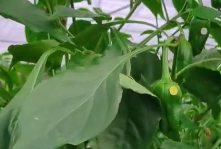
\includegraphics[width=\columnwidth]{images/png/ID2.png}
    \caption{Fruit (ID:2)}
    \label{Fig:id2}
  \end{minipage}
  \hspace{0.02\columnwidth}
  \begin{minipage}[b]{0.49\columnwidth}
    \centering
    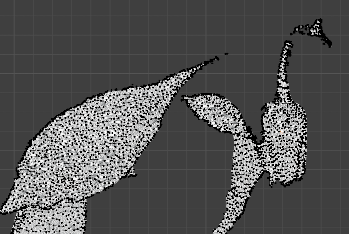
\includegraphics[width=\columnwidth]{images/png/ID2model.png}
    \caption{Fruit model (ID:2)}
    \label{Fig:id2model}
  \end{minipage}
\end{figure}